\section{\textsc{Постановка эксперимента на стенде СУРА}}

Нагревательный стенд СУРА (56,15\degree N, 46,1\degree E) был создан в 1981 году для проведения прикладных и фундаментальных исследований состояния ионосферы при воздействии на неё ВЧ излучением техногенного характера.  
Основу стенда составляют три ВЧ радиопередатчика, каждый из которых имеет мощность 250 кВт и работает в диапазоне частот 4-25 МГц, а также антенная решётка размером примерно $300\times300\,\text{м}^2$, которая позволяет излучать волны O- и X- поляризации в диапазоне частот 4,3-9,5 МГц. 
Эффективная мощность излучения (в случае синхронной работы трёх модулей) и ширина диаграммы направленности составляют 80-240 МВт и 6-12\degree, соответственно.  
Сканирование может выполняться в плоскости геомагнитного меридиана (наклонение геомагнитного поля в районе стенда 71\degree) в диапазоне $\pm40\degree$ от вертикали.     
С более подробным описанием стенда можно ознакомиться в работе \cite{Belikovich2007}.

В данной работе рассматриваются экспериментальные сеансы за три дня: 23 августа 2010 года, 19 и 20 сентября 2016 года. 
Их программа работы представлена в прил. \ref{ap-2}.
Эксперименты проводились в условиях дневной и вечерней ионосферы (по местному времени).
При этом использовались разные режимы работы стенда, начиная с [+90 c, -30 c] и заканчивая [+14 мин, -16 мин], где ``+'' означает длительность волны накачки (ВН), а ``-'' -- длительность паузы.  
Чтобы обеспечить резонансное взаимодействие с ионосферной плазмой, частота ВН была меньше или порядка критической частоты слоя F2. 
Помимо этого, сканирование выполнялось в плоскости геомагнитного меридиана под углом 12\degree~(от вертикали) к югу, чтобы усилить генерацию искусственной ионосферной возмущённости за счёт магнитного зенита \cite{Streltsov2018, Tereshchenko2004}.

Согласно работе \cite{Kunitsyn2012}, для сеансов 23 августа 2016 года максимальные значения вариаций TEC (0,5-0,7 TECU) наблюдались в случае использования волн O-поляризации в вечерние и ночные часы.
Поэтому именно это время является наиболее перспективным, где можно ожидать ухудшение точности позиционирования. 

Возможность формирования области искусственной ионосферной возмущённости на значительном расстоянии от нагревательного стенда связана с генерацией искусственных или усилением естественных ПИВ.
Согласно работам \cite{Chernogor2011, Chernogor2013, Kunitsyn2012}, подобные ПИВ наблюдаются преимущественно в вечерние часы при резонансной генерации ВН O-поляризации и модуляции эффективной излучаемой мощности с частотой меньше порядка частоты Брента-Вяйсяля на ионосферных высотах. 
Поэтому ухудшение точности позиционирования на значительном расстоянии от нагревательного стенда можно ожидать, где период модуляции эффективной излучаемой мощности примерно равен 20 мин и более.
Также необходимо учитывать, что в среднеширотной ионосфере амплитуды искусственных ПИВ обычно не превышают характерные амплитуды естественных ПИВ, особенно во время прохождения солнечного терминатора в области зондирования.

Геомагнитная обстановка в рассматриваемые дни была относительно спокойной.
23 августа 2010 года глобальный планетарный индекс геомагнитной активности $\text{Kp}=0,3\div3,7$, а индекс глобального симметричного экваториального тока $\text{SYM-H}=-1\div4$ нТл.
19-20 сентября 2016 года были более возмущенными днями: индекс Kp достигал значения 4,3 (20 сентября 00:03 UT), а индекс SYM-H дважды опускался до -37 нТл (19 сентября 10:30 UT и 20 сентября 02:30 UT).

В работе используются двухчастотные измерения GPS 14 приёмных станций, расположенных на различном расстоянии от нагревательного стенда СУРА.
Информация об используемых навигационных приёмниках представлена в прил. \ref{ap-3}, где также приведено их расстояние до области нагрева на высоте 250 км (55,7\degree N, 46,01\degree E).
Наиболее близкие приёмники были размещены на самом полигоне (SURA и PREG), а также на удалении до 20 км от него (ZASU и VORO).
Остальные 10 приёмников, входящие в сети SmartNet и TatNet, находились на расстоянии от 23 до 1217 км от стенда.  
Полная схема размещения используемых навигационных приёмников изображена на рис. \ref{fig-sites}.

В качестве изучаемой величины рассматривается полная ошибка позиционирования, которая вычисляется аналогично выражению \eqref{eq-3d-error}.
Помимо этого, в дополнение к двухчастотному кинематическому режиму PPP, реализуемому при помощи программного обеспечения с открытым исходным кодом GAMP \cite{Zhou2018}, используется обычный одночастотный режим (L1C код) с ионосферной коррекцией по модели Клобучара \cite{Klobuchar1987}. 
\clearpage
\begin{figure}[h]
\centering    
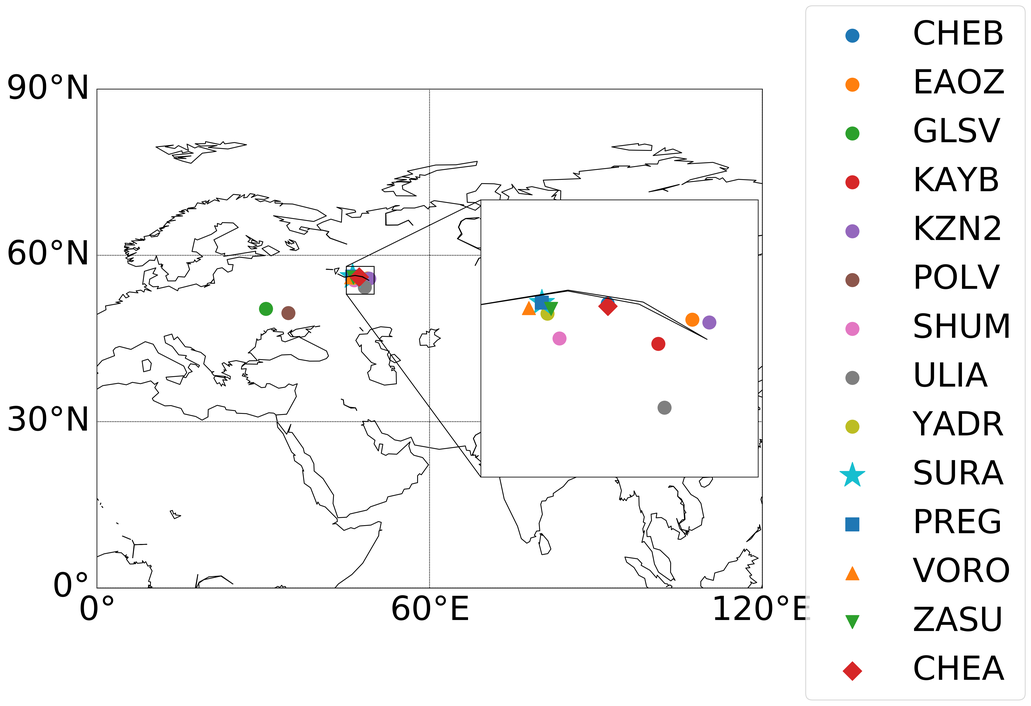
\includegraphics[width=0.7\textwidth]{fig/sites.png}    
\caption{Геометрия расположения навигационных приёмников, используемых в эксперименте.}
\label{fig-sites}      
\end{figure}  